The requirements for the product are prioritized using the MoSCoW method. Using this, the requirements for the product are divided into four sections, where the most important elements are given the highest priority. \textbf{Must} are the requirements that are an absolute necessity for the product. \textbf{Should} are the requirements that are also of high priority, but not quite mandatory. \textbf{Could} are requirements which may be met, if the time and other constraints of the project allow for it. \textbf{Won't} are the requirements the product will not meet, but could be developed at a later point in its lifetime.  

\noindent The following priorities have been chosen for this project:
\begin{itemize}
	\item[\textbf{Must}]
		\begin{itemize}
			\item Navigate waypoints from user input
			\item Be compatible with NMEA protocol GPS input
			\item Use GPS for localization
			\item Implement a PID control loop
		\end{itemize}
	\item[\textbf{Should}]
		\begin{itemize}
			\item Control thrusters in two-thruster catamaran
			\item Use a graphical user interface for user interaction
			\item Be able to change the PID parameters
		\end{itemize}
	\item[\textbf{Could}] 
		\begin{itemize}
			\item Control wheel in outboard motor on boat
			\item Be generic enough to use with other engine types
		\end{itemize}
	\item[\textbf{Won't}]
		\begin{itemize}
			\item Use pylogon-coverage for a specified area
			\item Avoid obstacles
		\end{itemize}
\end{itemize}

The following two diagrams specify the actor context to the system, and the use cases for the system.

\begin{figure}[H]
	\centering
	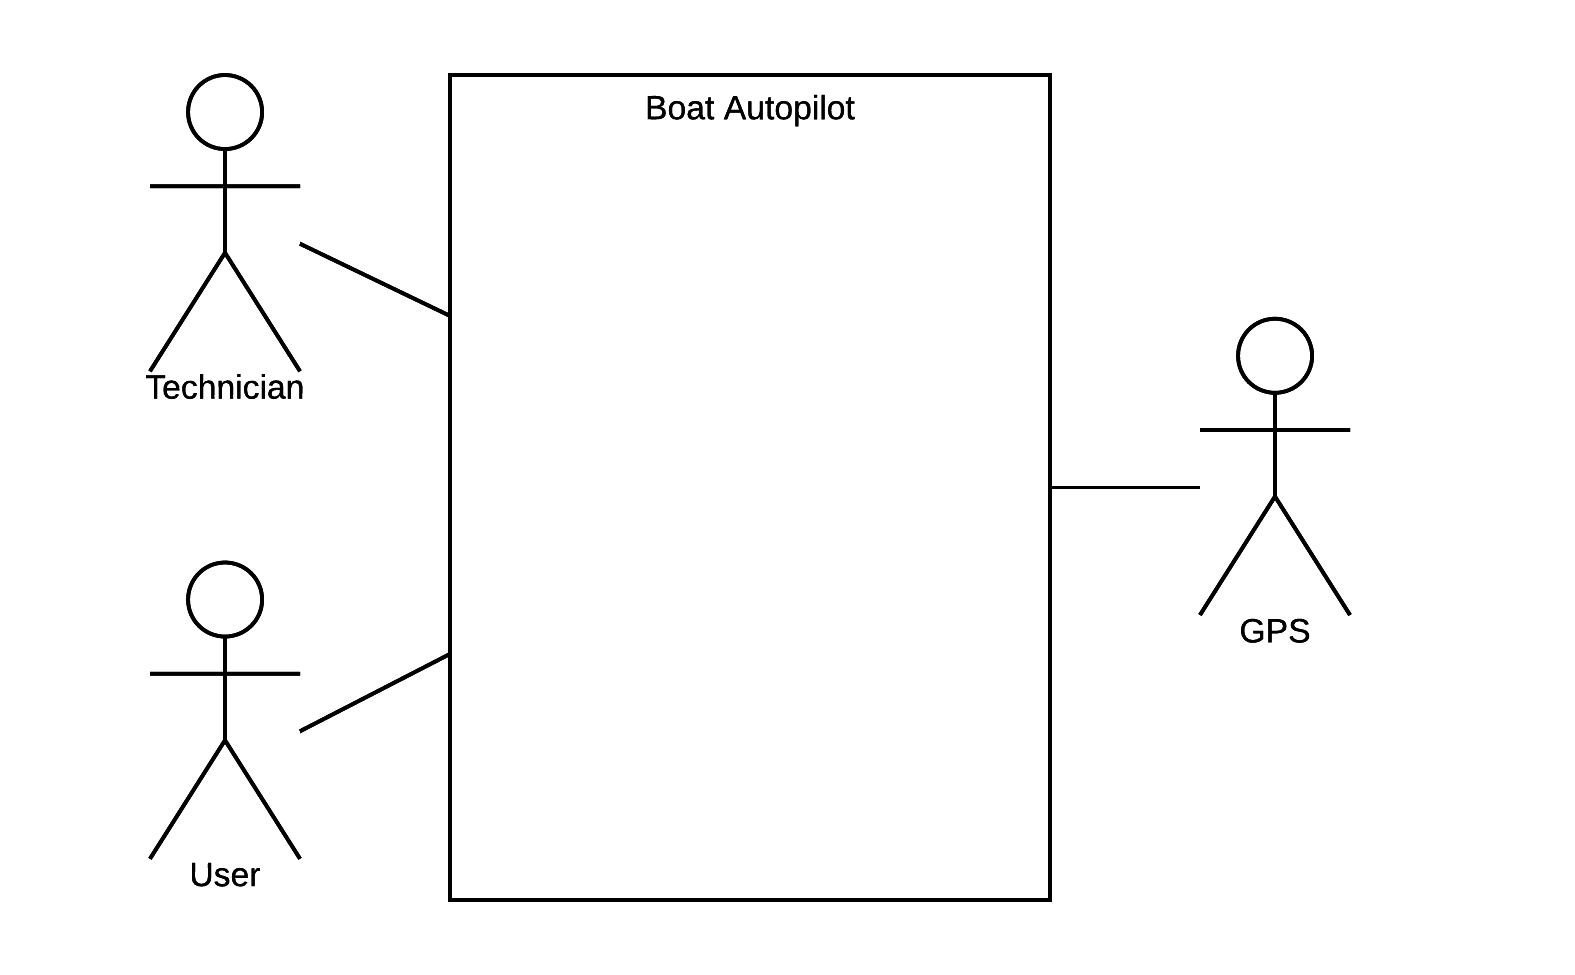
\includegraphics{Images/Actor_context_diagram.png}
	\caption{Actor context diagram}
\end{figure}

\begin{figure}[H]
	\centering
	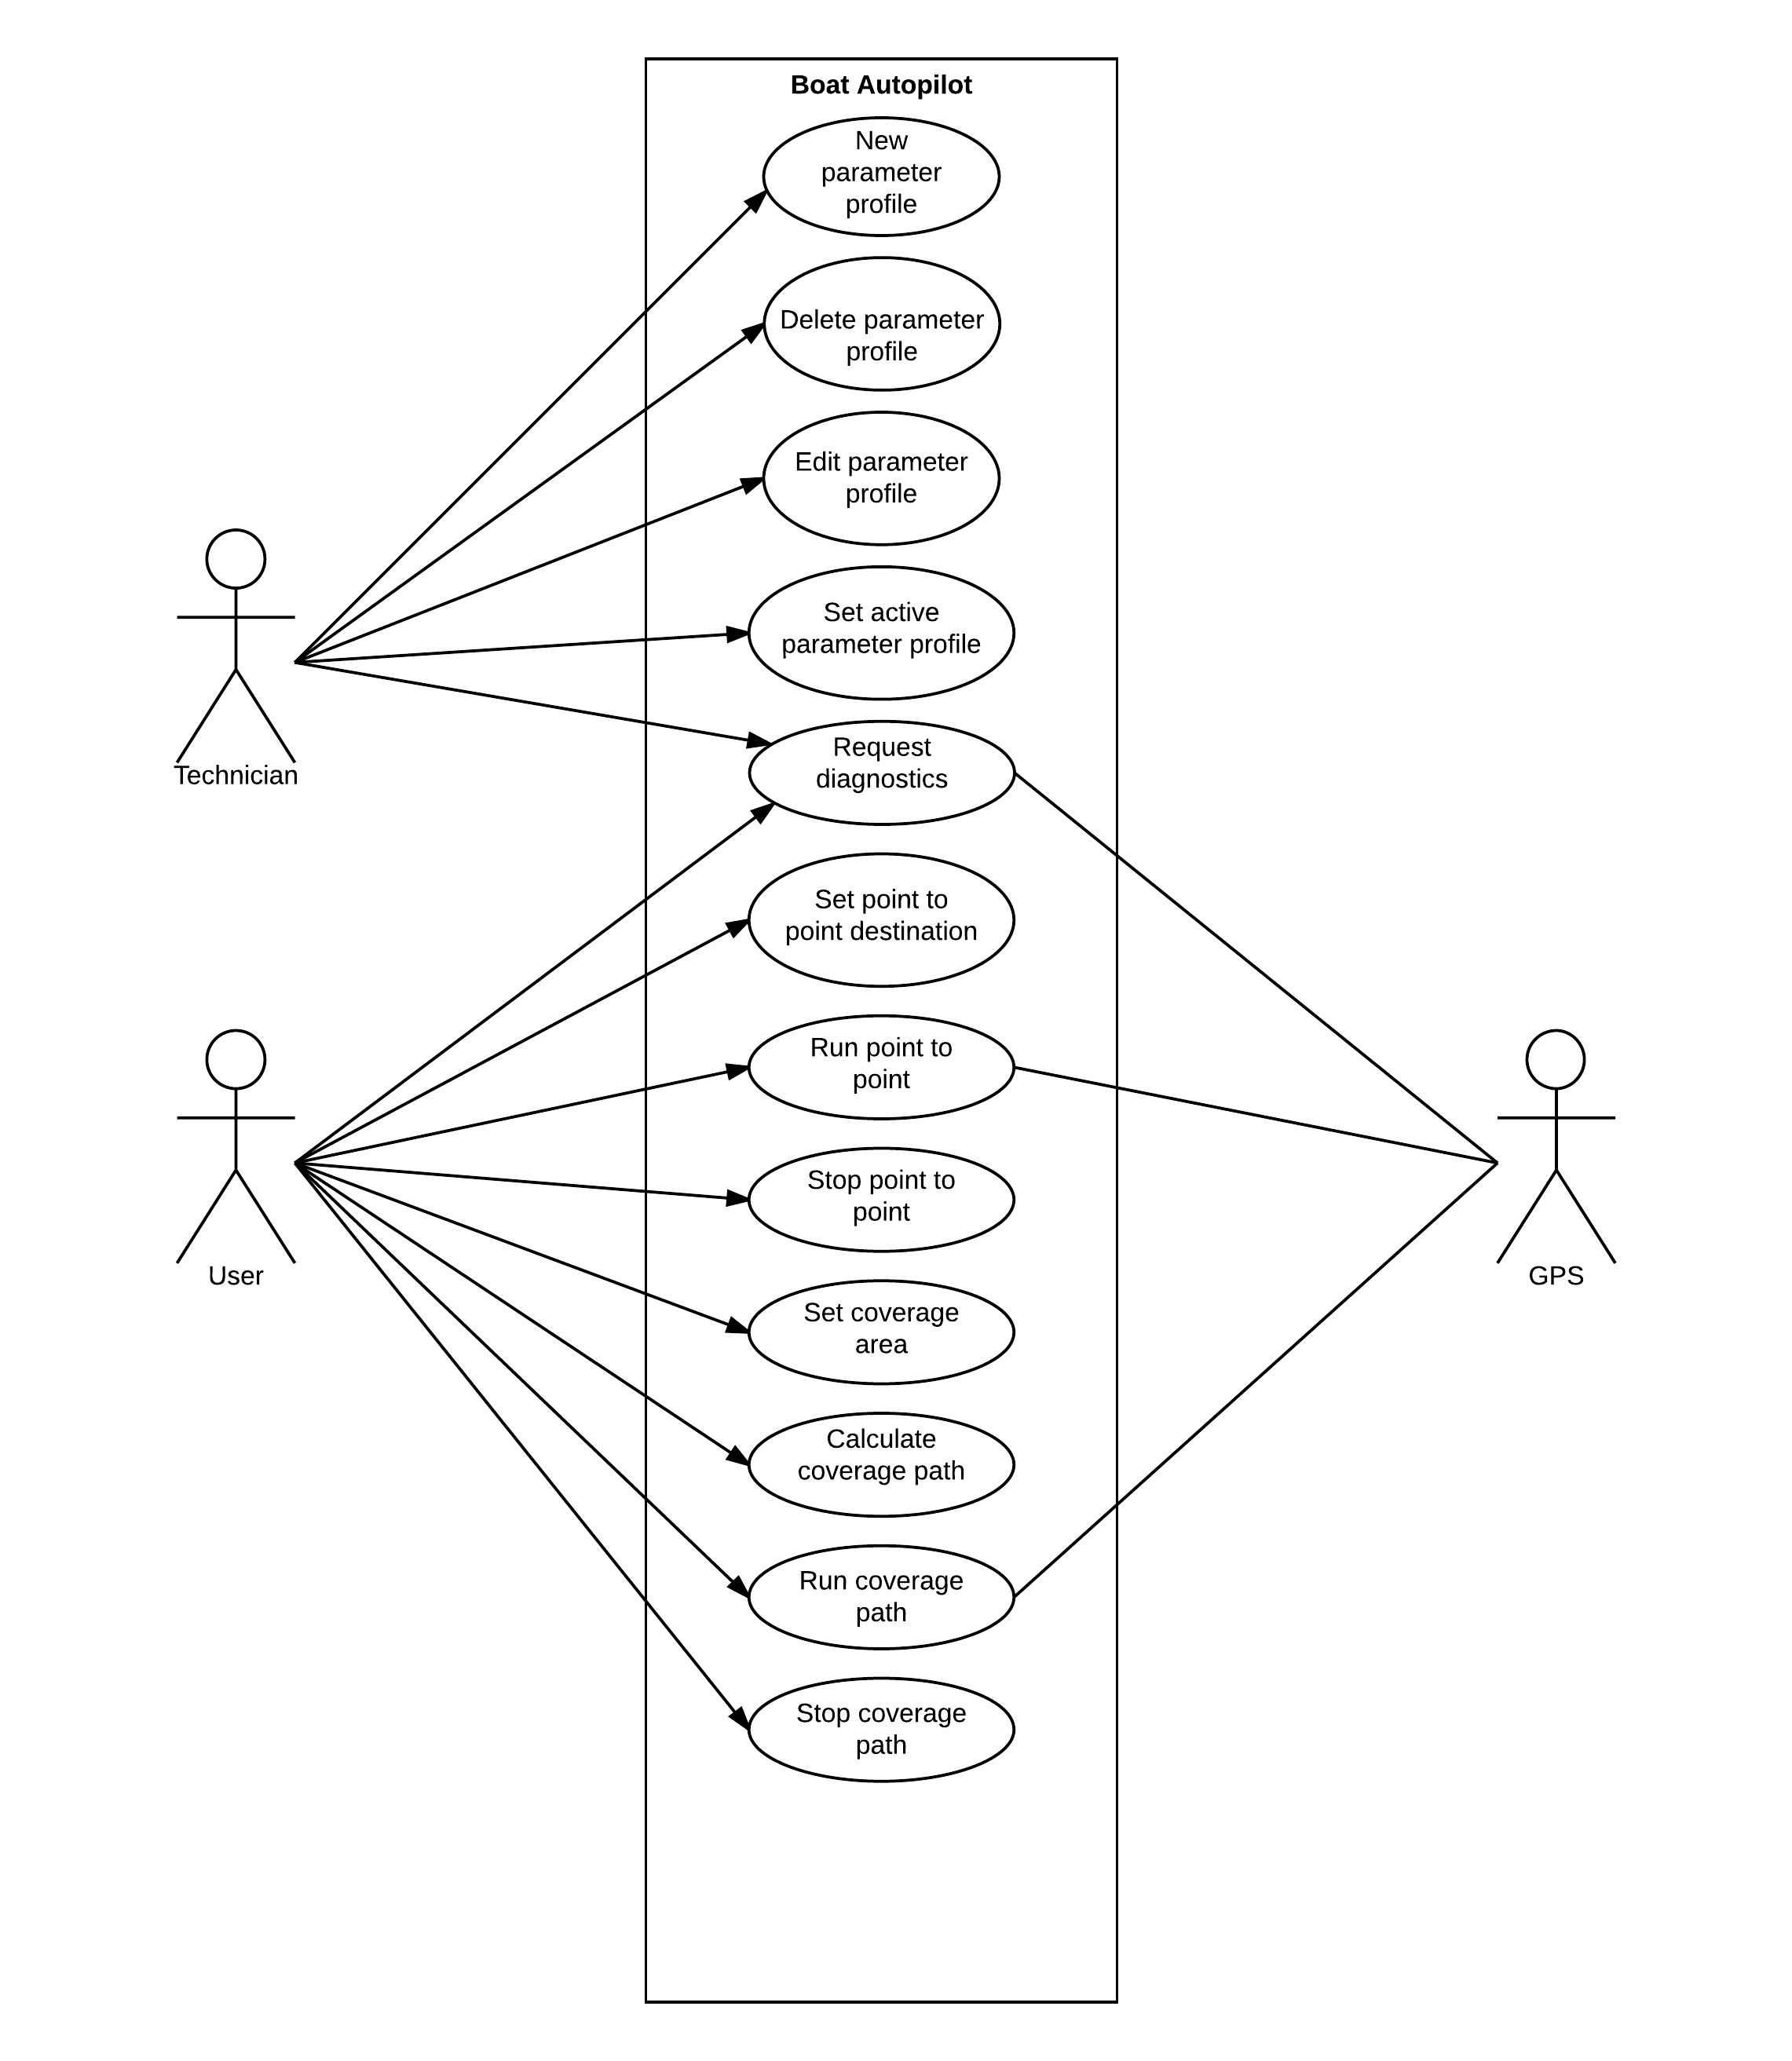
\includegraphics[width=0.9\linewidth]{Images/Usecase_diagram}
	\caption{Use case diagram}
	\label{fig:usecasediagram}
\end{figure}


\section{Actor description}
The following section describes the system's actors. Every actor has a type and a short description of its function and impact on the system.

\begin{framed}
	\subsection{Actor: Technician}
	\subsubsection*{Type:}
	Primary
	
	\subsubsection*{Description:}
	A technician with knowledge of the system. This actor triggers the use case "Specify parameters".
	
\end{framed}

\begin{framed}
	\subsection{Actor: User}
		\subsubsection*{Type:}
			Primary
	
		\subsubsection*{Description:}
			The user, or customer. This actor triggers the use case "Specify waypoints".
\end{framed}

\begin{framed}
	\subsection{Actor: GPS}
		\subsubsection*{Type:}
			Secondary
	
		\subsubsection*{Description:}
			The global positioning system. This actor assists in carrying out the use case "Navigate waypoints".
	
\end{framed}

\pagebreak

\section{Use cases}

\subsection{Use case 1 - Enter parameters}
\subsubsection*{Goal:}
To enter the parameters for the boat being used.

\subsubsection*{Initialization:}
Technician

\subsubsection*{Actors:}
Technician (primary)

\subsubsection*{References:}
None

\subsubsection*{Simultaneous occurances:}
One

\subsubsection*{Prerequisite:}
None

\subsubsection*{Result:}
The autopilot parameters have been updated.

\subsubsection*{Main scenario:}
\begin{enumerate}
	\item The technician investigates the boat which will be used, specifically its drive system.
	\item The boat parameters are set using the graphical user interface. 
\end{enumerate}	
\end{framed}


\begin{framed}
	\subsection{Use case 1 - Enter parameters}
	\subsubsection*{Goal:}
		To enter the parameters for the boat being used.
		
	\subsubsection*{Initialization:}
		Technician
	
	\subsubsection*{Actors:}
		Technician (primary)
	
	\subsubsection*{References:}
		None
	
	\subsubsection*{Simultaneous occurances:}
		One
	
	\subsubsection*{Prerequisite:}
		None
	
	\subsubsection*{Result:}
		The autopilot parameters have been updated.
	
	\subsubsection*{Main scenario:}
		\begin{enumerate}
			\item The technician investigates the boat which will be used, specifically its drive system.
			\item The boat parameters are set using the graphical user interface. 
		\end{enumerate}	
\end{framed}

\begin{framed}
	\subsection{Use case 2 - Specify waypoints}
	\subsubsection*{Goal:}
	To enter waypoints, outlining a desired path through an area.
	
	\subsubsection*{Initialization:}
	User
	
	\subsubsection*{Actors:}
	User (primary)
	
	\subsubsection*{References:}
	None
	
	\subsubsection*{Simultaneous occurances:}
	One
	
	\subsubsection*{Prerequisite:}
	Use case 1 - Enter parameters has been completed.
	
	\subsubsection*{Result:}
	Waypoints for the path have been set.
	
	\subsubsection*{Main scenario:}
	\begin{enumerate}
		\item The user accesses the graphical user interface and sets a series of waypoints, detailing a path through the area starting at Waypoint 1.
	\end{enumerate}	
\end{framed}

\begin{framed}
	\subsection{Use case 3 - Navigate waypoints}
	\subsubsection*{Goal:}
	To navigate the set waypoints, outlining a desired path through an area.
	
	\subsubsection*{Initialization:}
	User
	
	\subsubsection*{Actors:}
	User (primary), 
	
	\subsubsection*{References:}
	None
	
	\subsubsection*{Simultaneous occurances:}
	One
	
	\subsubsection*{Prerequisite:}
	Use case 2 - Specify waypoints has been completed.
	
	\subsubsection*{Result:}
	The boat has completed its path through each waypoint.
	
	\subsubsection*{Main scenario:}
	\begin{enumerate}
		\item The user accesses the graphical user interface and selects "Start".
		\item The Boat Autopilot updates its current location using GPS signals.
		\item The Boat Autopilot begins navigating to the first waypoint using a feedback control loop, and continues this until each waypoint has been visited. The Boat's location is updated throughout using GPS.
	\end{enumerate}	
\end{framed}
